% !TeX encoding = UTF-8
% !TeX spellcheck = ru_RU
\section{Экспоненциальное распределение. Эффект без памяти}
Человек решил позвонить по телефону в момент времени $ 0 $. Но не дозвонился.
Так же безуспешно он пытался дозвониться t1 времени. Спустя $ T{*} $ времени после $ t1 $ человек дозвонился. 

\begin{center}
	$M[T^{*}]=M[T\vert T>t1]=\frac{1}{\lambda}$
\end{center}

\subsection{Постановка задачи}
Написать моделирующую программу (провести имитационное моделирование)
для данной ситуации. Показать, что утверждение справедливо только
в том случае, если случайная величина распределена по экспоненциальному
закону. 

\subsubsection{Пример}
Пусть автобусы приходят на остановку случайно, но с некоторой фиксированной
средней интенсивностью. Тогда количество времени, уже затраченное
пассажиром на ожидание автобуса, не влияет на время, которое ему ещё
придётся прождать. 

Пусть случайная величина $ R $ распределена по экспоненциальному закону. Тогда верно следующее неравенство:
\[ P{r}\{R>a+b | R>=a\}=Pr\{R>b\} \]

Для демонстрации данного эффекта сгенерируем $n$ случайных величин
$r_{i}\sim Exp(\lambda),i=1,n$ . Вычислим математическое
ожидание и дисперсию как \[ M[R]=\frac{\sum_{i=1}^{n}x_{i}}{n} \]
и \[ D[R]=\frac{\sum_{i=1}^{n}r_{i}^{2}}{n}-M[R]^{2} \]. Получим, что $M[R]=\frac{1}{\lambda}, D[R]=\frac{1}{\lambda^{2}}$. Затем получим случайную величину $R^{'}$ как $r_{i}^{'}=r_{i}-t_{k}$ и оставим только те значения для которых верно неравенство $r^{'}\geq0$. Пусть количество этих новых значений равно $n^{'}$. Вычислив $M[R^{'}]$
и $D[R^{'}]$ получим, что \[ M[R]=M[R^{'}] \]
\[ D[R]=D[R^{'}] \]

Сгенерирована случайная величина $R,$ $r_{i}\sim Exp(\lambda),i=1,n$
распределенная по экспоненциальному закону, количество элементов последовательности
$n=10000$, $\lambda=0,5$ . 

\begin{figure}[h]
	\centering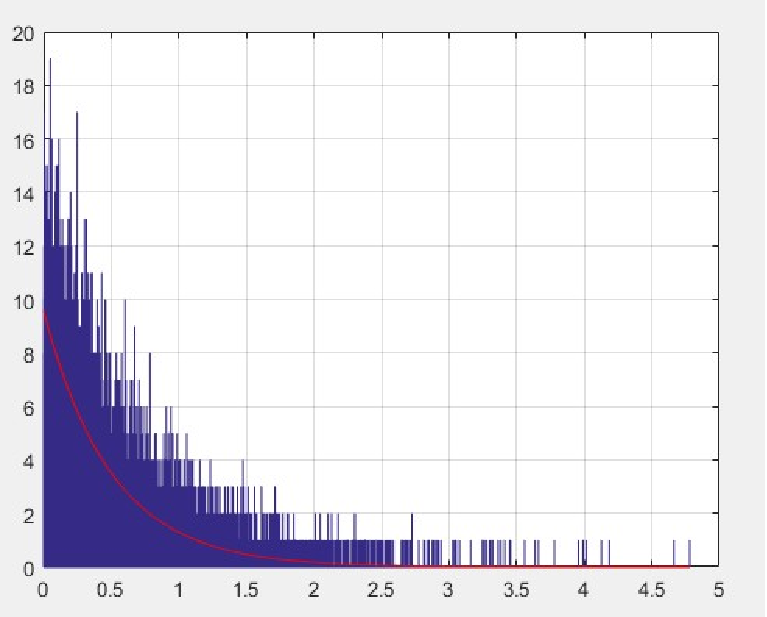
\includegraphics[width=0.4\linewidth]{img/kich_bur/image1}
	\caption{Гистограмма случайной величины $ R $, $r_i \sim Exp(\lambda),i=(1,n) $ распределенная по экспоненциальному закону, количество элементов последовательности $ n=10000, \lambda=0,5 $}
	\label{fig:img1}
\end{figure}

$Exp(\lambda),i=1,n$
распределенная по экспоненциальному закону, количество элементов последовательности
$n=10000$, $\lambda=0,5$ 


Мат.ожидание случайной величины $ R $ распределенной по экспоненциальному
закону = $ 0.5009  $

Дисперсия случайной величины $ R $ распределенной по экспоненциальному
закону = $ 0.2532 $ 

Получим величину $R^{'}$ как $r_{i}^{'}=r_{i}-t_{1}$ и оставим
только те значения, которые $r^{'}\geq0$ . Пусть количество этих
новых значений равно $n^{'}$ . Пусть $t_{1}=0.7$

\begin{figure}[h]
	\centering
	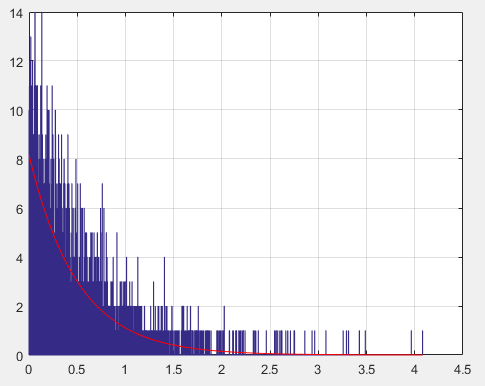
\includegraphics[width=0.4\linewidth]{img/kich_bur/image2}
	\caption{Гистограмма случайной величины $ R^{'} $}
	\label{fig:img2}
\end{figure}

\begin{figure}[h]
	\centering
	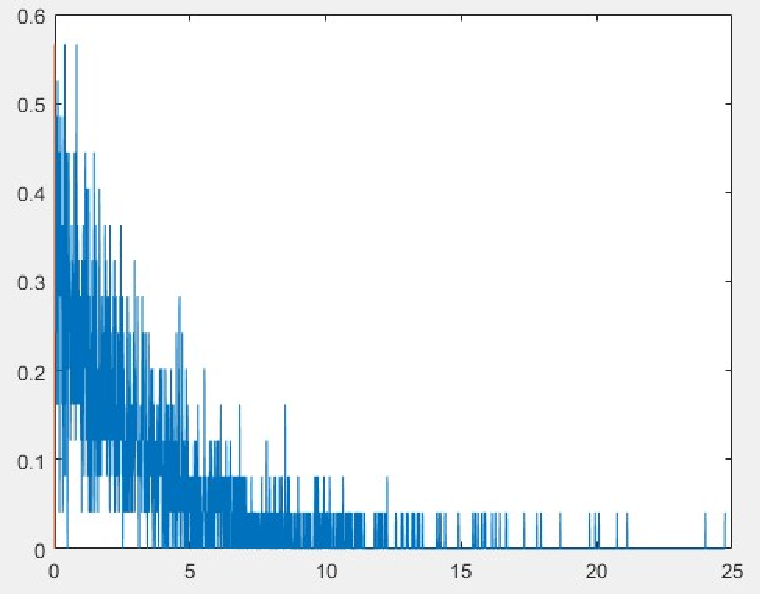
\includegraphics[width=0.4\linewidth]{img/kich_bur/image3}
	\caption{График плотности вероятности случайной величины $ R^{'} $}
	\label{fig:img3}
\end{figure}

$M[R^{'}]= 0.5024$

Количество элементов на второй итерации $n^{'}=2473$

Дисперсия на второй итерации $D[R^{'}] = 0.2587 $

Получим величину $R^{''}$ как $r_{i}^{''}{}^ {}=r_{i}^{'}-t_{2}$
и оставим только те значения, которые $r^{''}\geq0$. Пусть количество
этих новых значений равно $n^{''}$. Пусть $t_{2}=0.3.$ 
\begin{figure}[h]
	\centering\
	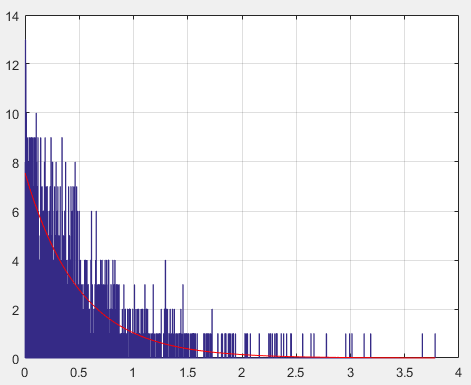
\includegraphics[width=0.4\linewidth]{img/kich_bur/image4}
	\caption{Гистограмма случайной величины $R^{''}$ }
	\label{fig:img4}
\end{figure}

Мат.ожидание после шага 2: $M[R^{''}]= 0.4947 $

Количество элементов на второй итерации: $n^{''}= 1381 $

Дисперсия на третьей итерации: $D[R^{''}]= 0.2638 $

Для сравнения проведем аналогичный опыт, сгенерировав последовательность
по закону Пуассона. Сгенерирована случайная величина $ RN $, $rn_{i}\sim
P(\lambda),i=1,n$ распределенная по закону Пуассона, количество элементов
последовательности $n=10000$, $\lambda=4$.
 
\begin{figure}[h]
	\centering
	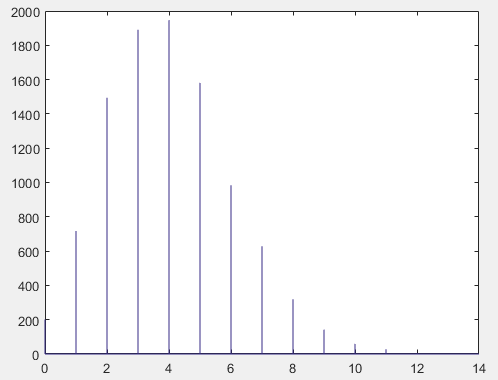
\includegraphics[width=0.4\linewidth]{img/kich_bur/image5} 
	\caption{Гистограмма случайной величины распределенной по закону Пуассона}
	\label{fig:img5}
\end{figure}

Сравним результаты. Для экспоненциального распределения: 

$M[R]= 4.0269$ 

$D[R]= 15.8816$ 

Мат.ожидание для распределения по закону Пуассона: 

$M[RN]= 4.0212$ 

Дисперсия для распределения по закону Пуассона: 

$D[RN]= 4.1518$ 

Получим величину $R^{'}$ и $RN^{'}$ как $r_{i}^{'}=r_{i}-t_{1}$
и $rn_{i}^{'}=rn_{i}-t_{1}$ оставим только те значения, которые
${r^{'}}$ и ${rn^{'}\geq0}$. Пусть количество этих новых
значений равно $n^{'}$ и $nr^{'}$ . Пусть $t_{1}=0.7.$ 

$M[R']= 4.0471$ 

количество элементов на второй итерации: 

$n'= 8366$ 

дисперсия на второй итерации: 

$D[R^{'}]=15.8007$

$M[RN']= 3.4033$ 

$D[RN']= 3.8984$ 

Для сравнения проведем аналогичный опыт, сгенерировав последовательность
по равномерному закону. Сгенерирована случайная величина RR, $rr_{i}\sim P(n),i=1,n$
распределенная по равномерному закону, количество элементов последовательности
$ n=10000  $
\begin{figure}[h]
	\centering
	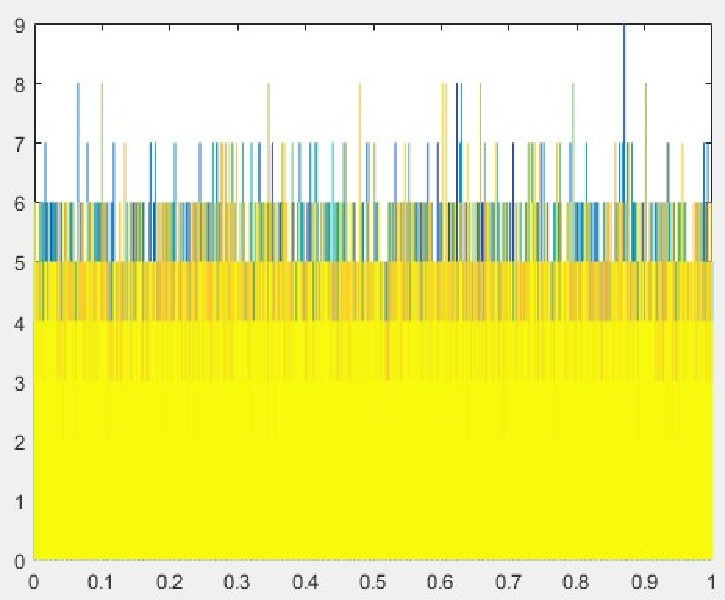
\includegraphics[width=0.4\linewidth]{img/kich_bur/image6} 
	\caption{Гистограмма случайной величины $RR$ }
	\label{fig:img6}
\end{figure}

Мат.ожидание для распределения по равномерному закону $M[RR]=0.4906$ 

Дисперсия для распределения по равномерному закону $D[RR]=
0.0834 $

Мат.ожидание после шага 1 по равномерному закону $M[RR']=
0.1472 $

Количество элементов на второй итерации по равномерному закону $n'=
295 $

Дисперсия на второй итерации по равномерному закону \[ D[RR^{'}]=0.0075 \]
\begin{figure}[h]
	\centering
	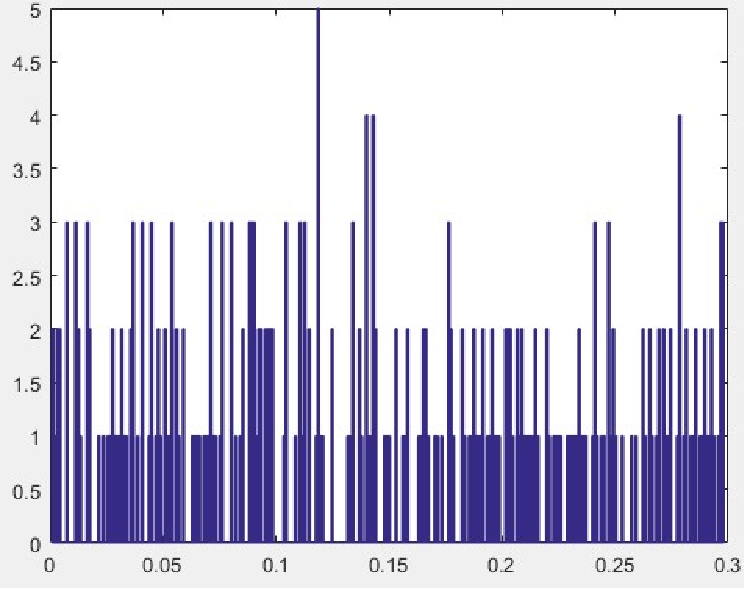
\includegraphics[width=0.4\linewidth]{img/kich_bur/image7} 
	\caption{Гистограмма случайной величины $RR^{'}$}
	\label{fig:img7}
\end{figure}

Сгенерируем две последовательности распределенные по
экспотенциалному закону по n случайных величин:  $R,$
$rd_{i}\sim Exp(\lambda)+sim Exp(\lambda),i=1,n$.
Вычисли мат.ожидание и дисперсию. Затем получим случайную величину $Rd^{'}$ как
$rd_{i}^{'}=rd_{i}-t_{1}$ и оставим только те значения, которые $rd^{'}\geq0$ .
Пусть количество этих новых значений равно $nd^{'}$ . Пусть $t_{1}=0.7$

Мат.ожидание суммы двух случайных величин $ Rd $ распределенных по
экспоненциальному закону = $ 8.3967  $

Дисперсия суммы двух случайных величин $ Rd $ распределенных по
экспоненциальному закону = $ 34.2300 $ 
\[ M[Rd^{'}]= 7.7769; D[Rd^{'}]= = 33.9038; nd^{'}= 990 \]
 

\subsection{Выводы}

\[ M[R]= 0.5009; D[R]= 0.2532  \]


\[ M[R^{'}]= 0.5024; D[R^{'}]= = 0.2587 \]


\[ M[R^{''}]= 0.4947; D[R^{''}]= 0.2638 \]


\[ M[RN]= 4.0212; D[RN]=4.1518 \]


\[ M[RN']= 3.4033; D[RN']= 3.8984 \]


\[ M[RR]= 0.4906; D[RR]= 0.0834 \]


\[ M[RR']= 0.1472; D[RR']= 0.0075 \]

\[ M[Rd]= 8.3967; D[Rd]= 34.2300 \]

\[ M[Rd^{'}]= 7.7769; D[Rd^{'}]= 33.9038 \]

Вычислив $M[R^{'}]$ и $D[R^{'}]$ получим, что:
\[ M[R]=M[R^{'}]\]
\[D[R]=D[R^{'}] \]

Таким образом, для случайной величины распределенной по экспоненциальному
закону, эффект отсутствия памяти работает. Утверждение справедливо
только в том случае, если случайная величина распределена по экспоненциальному
закону, что соответствует теории и результатам моделирования. Сумма двух
случайных величин, распределенных по экспоненциальному закону, данным эффектом не
обладает.

Код программы на Matlab [\ref{code:code1}]:
%\lstinputlisting[language=Matlab, label=code:code1, captionpos=b, caption=Программа моделирования]{src/1.m}
\newpage